\section{Small stereo roads}
\label{sec:stereoroads}
\begin{figure}[!htpb]
  \begin{center}
    \includegraphics[width=0.48\textwidth]{figures/cartoon_roads_small_smallstereo_1.pdf}
    \includegraphics[width=0.48\textwidth]{figures/cartoon_roads_large_smallstereo_1.pdf}
  \end{center}
  \vspace{-10pt}
  \caption{Sketch of the road coverage of the proposed MMTP algorithm, for a small chamber closest to the beamline (left) and large chamber farthest from the beamline (right). The $X$ road is horizontal, the $U$ road is pink and slanted, and the $V$ road is blue and slanted. For ease of digestion, only one pair of $U$ and $V$ roads are shown, and they do not cover the entire $X$ road. The x-axis and y-axis are in units of strip pitches, which are 0.4 mm.}
  \label{fig:cartoon_smallroads_1}
\end{figure}
\begin{figure}[!htpb]
  \begin{center}
    \includegraphics[width=0.48\textwidth]{figures/cartoon_roads_small_smallstereo_N.pdf}
    \includegraphics[width=0.48\textwidth]{figures/cartoon_roads_large_smallstereo_N.pdf}
  \end{center}
  \vspace{-10pt}
  \caption{Sketch of the road coverage of the proposed MMTP algorithm, for a small chamber closest to the beamline (left) and large chamber farthest from the beamline (right). The $X$ road is horizontal, the $U$ roads are pink and slanted, and the $V$ roads are blue and slanted. The small chamber requires five pairs of $U$ and $V$ roads to cover one $X$ road, and the large chamber requires 19. The x-axis and y-axis are in units of strip pitches, which are 0.4 mm.}
  \label{fig:cartoon_smallroads_N}
\end{figure}
Due to the degraded performance of the nominal algorithm given a high uncorrelated background rate, we propose a modified, improved version of the algorithm.
We can divided each large $U$,$V$ road into multiple roads that are the same size as the $X$ road. Then, each $X$ road has multiple associated $U$,$V$ roads. The overlap of one set of these roads forms a single diamond, which is illustrated in Figure \ref{fig:cartoon_smallroads_1}. To span the length of the chamber, we have a cascade of diamonds, illustrated in Figure \ref{fig:cartoon_smallroads_N}. This dramatically narrows the spatial region in which a coincidence is found. This also reduces the chance that a muon track hit is overwritten by a background hit. Note that it is important that the coincidence threshold be at least 3 X-planes and 3-U,V planes to reduce background triggers. The background rate goes with the $\text{hit rate per plane}^{\text{number of planes}}$.  
\par The performance of the improved algorithm is shown in Figure \ref{fig:resolutions_new}. As expected, the x-resolution is comparable to that of the nominal algorithm, but the y-resolution shows a dramatic improvement. The 3$\sigma$ RMS is 11.29 (12.68) $\pm$ 0.01 (0.01) mm for 0.5m (2.2m) long strips.The y-residual bounds go with the effective $U$,$V$ road size divided by the tangent of the stereo angle. We can also look at the efficiency of a $\Delta \phi <$ 20 mrad cut as a function of the uncorrelated background rate for both algorithms. In Figure \ref{fig:eff_vs_rate}, we see that the performance of the nominal algorithm drops sharply with increased background, while the proposed algorithm maintains 80\% (95\%)+ efficiency for up to a 60 kHz/strip background rate with 0.5m (2.2m) long strips.
\par We now elaborate on the use of implementation regions. It is important to divide the wedge into reasons so that each implementation of the firmware has a minimum number of triggers to process at any given time. There will be hard limit to how many triggers can be processed per BC per implementation. Thus, small implementation regions are ideal. As a technical aside, the exact number of roads in an implementation region is presently determined by the architecture of the MMTP firmware. \footnote{The MMTP relies on multiplexers to select the $U$,$V$ roads overlapping with each $X$ road. If we consider the LM2 with a pitch of 450 microns, we have $2.2\text{m} \times \tan 1.5^\circ \times \frac{1}{450 \;\mu m \times 8 \text{ strips/road}} = 16 + 1$ $U$,$V$ roads associated to one $X$ road, so we need 17 multiplexers. Assuming standard multiplexer of 8:1, we can have 136 $X$ roads in the largest R region. A similar calculation can be done for the 0.5m strips.} 

\begin{figure}[!htpb]
  \begin{center}
    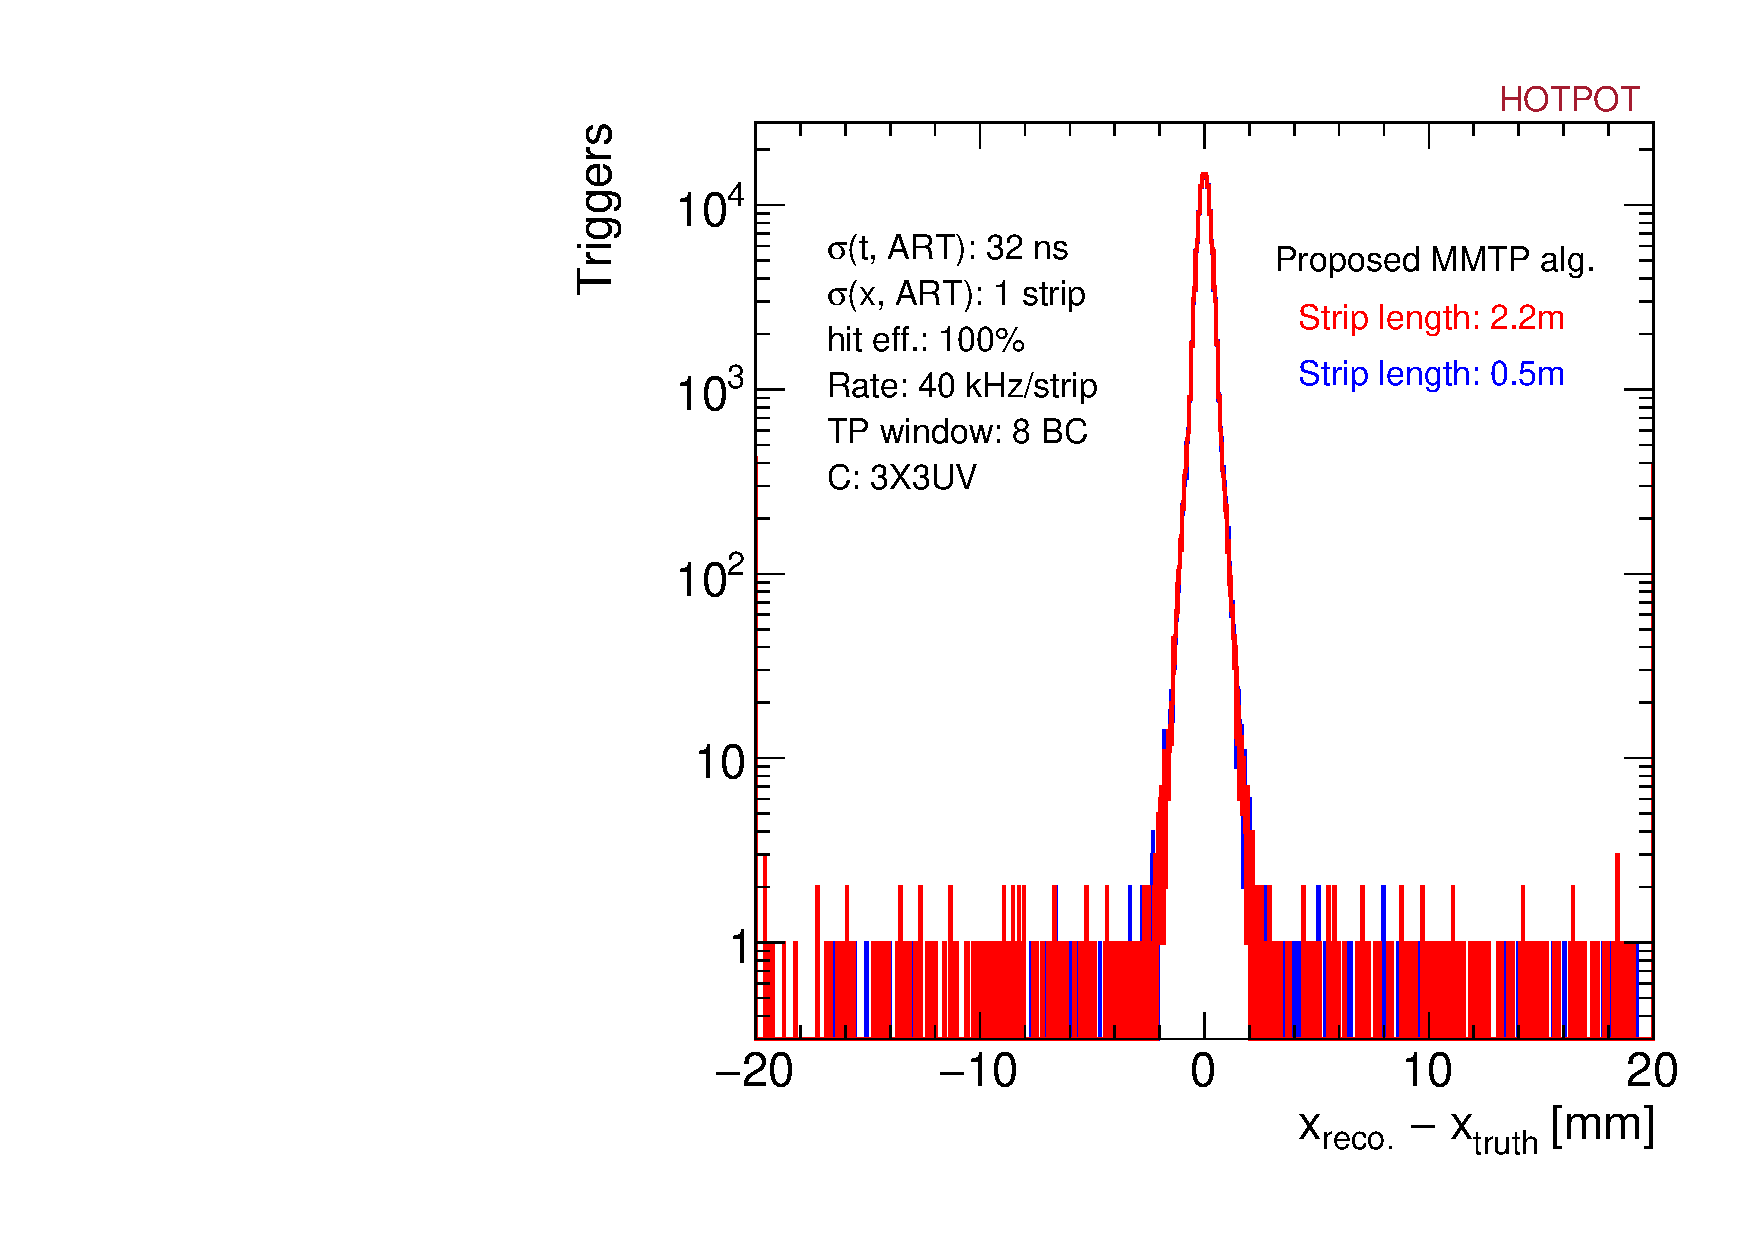
\includegraphics[width=0.48\textwidth]{figures/xres_new.pdf}
    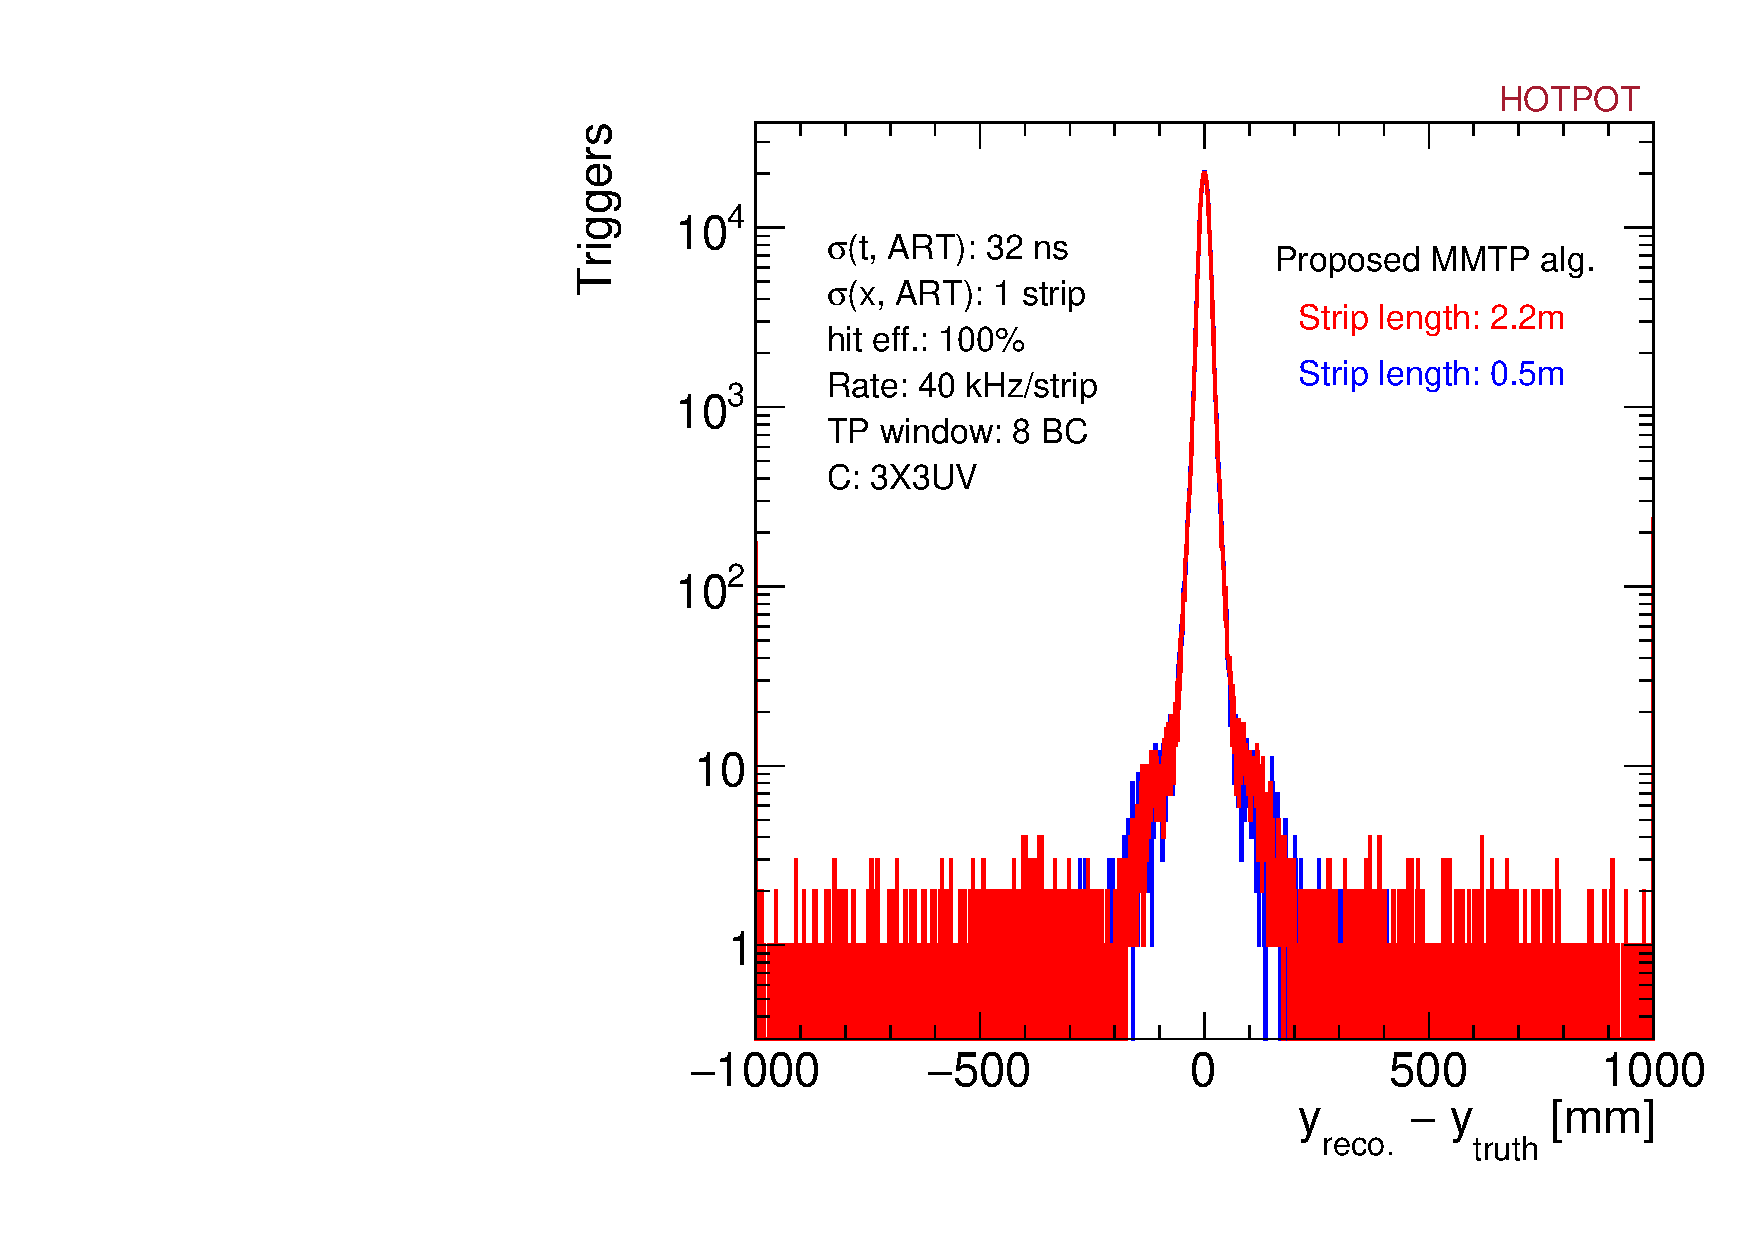
\includegraphics[width=0.48\textwidth]{figures/yres_new.pdf}
    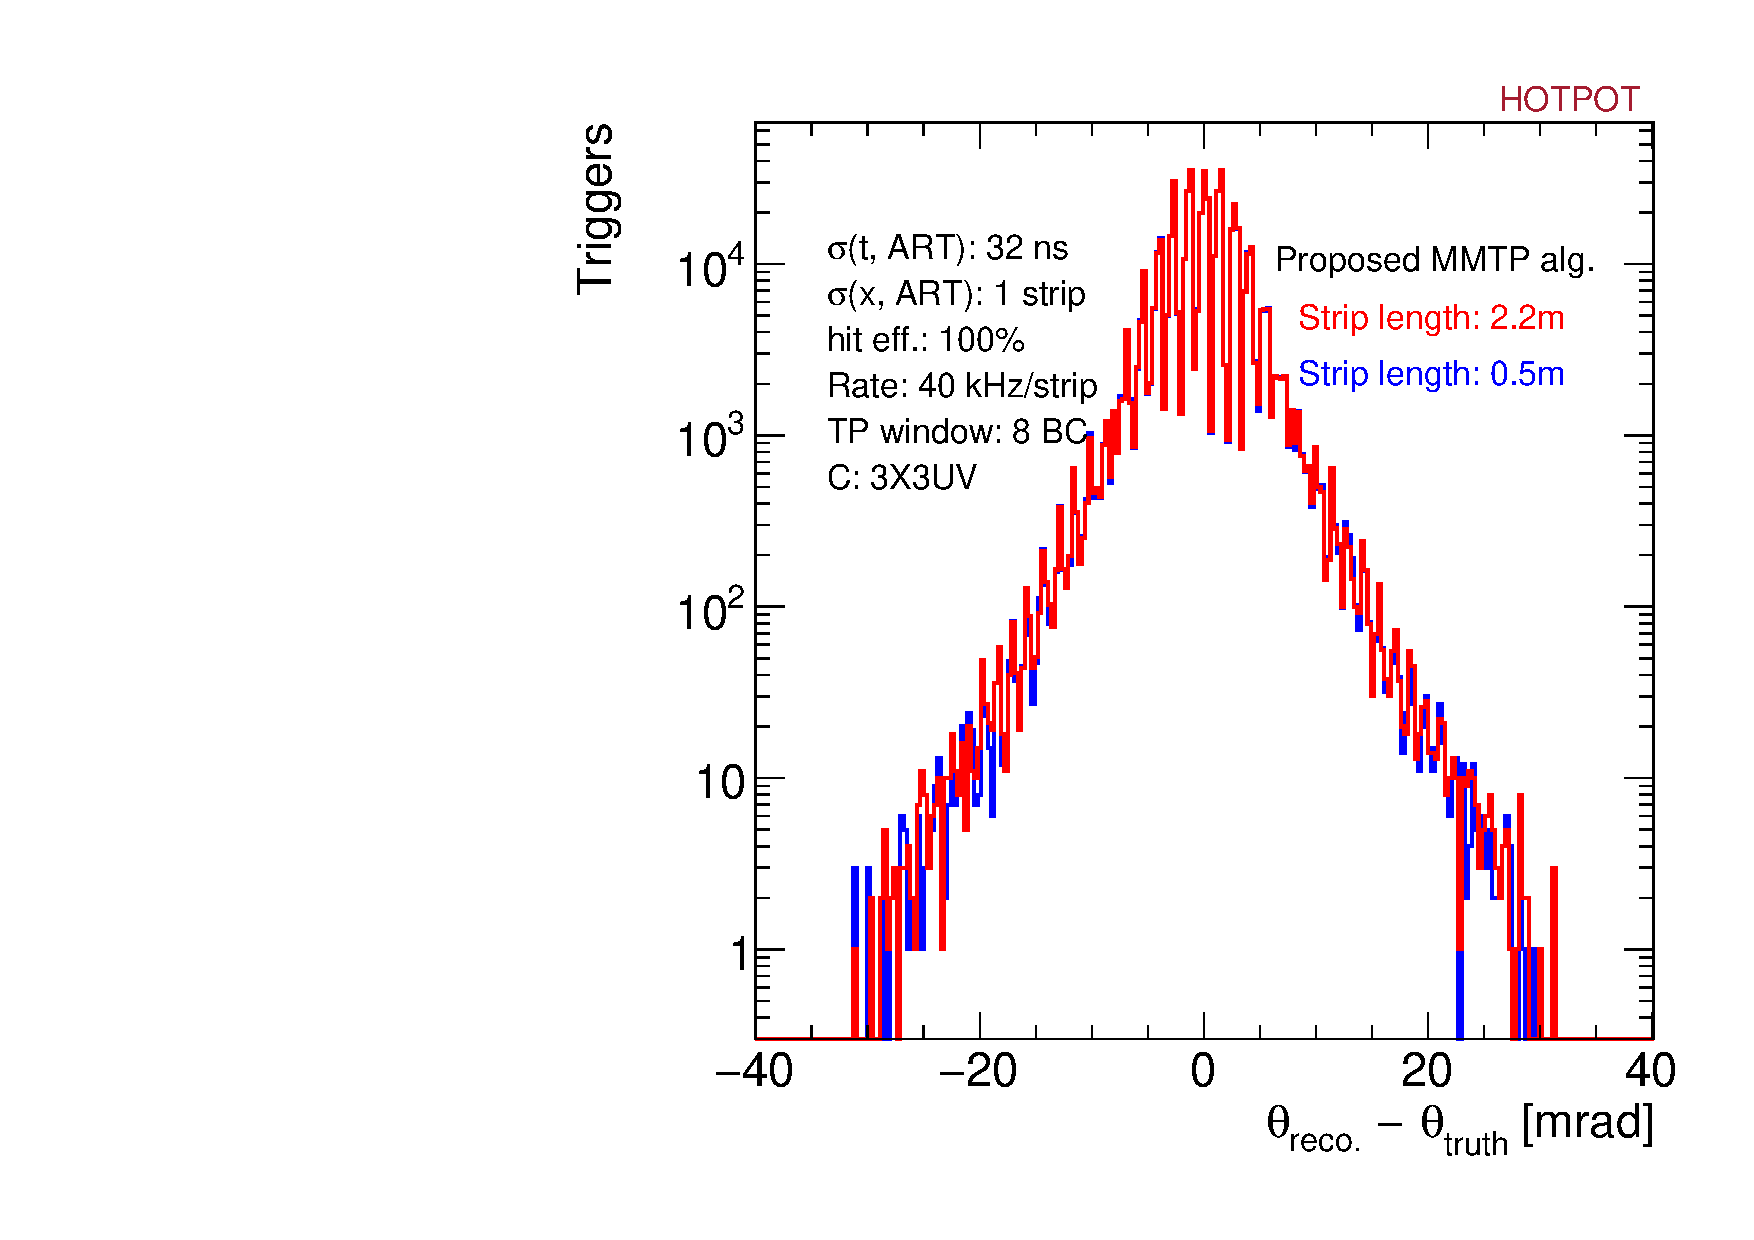
\includegraphics[width=0.48\textwidth]{figures/mres_new.pdf}
  \end{center}
  \vspace{-10pt}
  \caption{Distribution of $x_\text{reco.} - x_\text{truth}$ (top, left), $y_\text{reco.} - y_\text{truth}$ (top, right) and $\theta_\text{reco.} - \theta_\text{truth}$ (bottom) for the proposed MMTP algorithm with uncorrelated background at a rate of 40 kHz per strip.}
  \label{fig:resolutions_new}
\end{figure}

\begin{figure}[!htpb]
  \begin{center}
    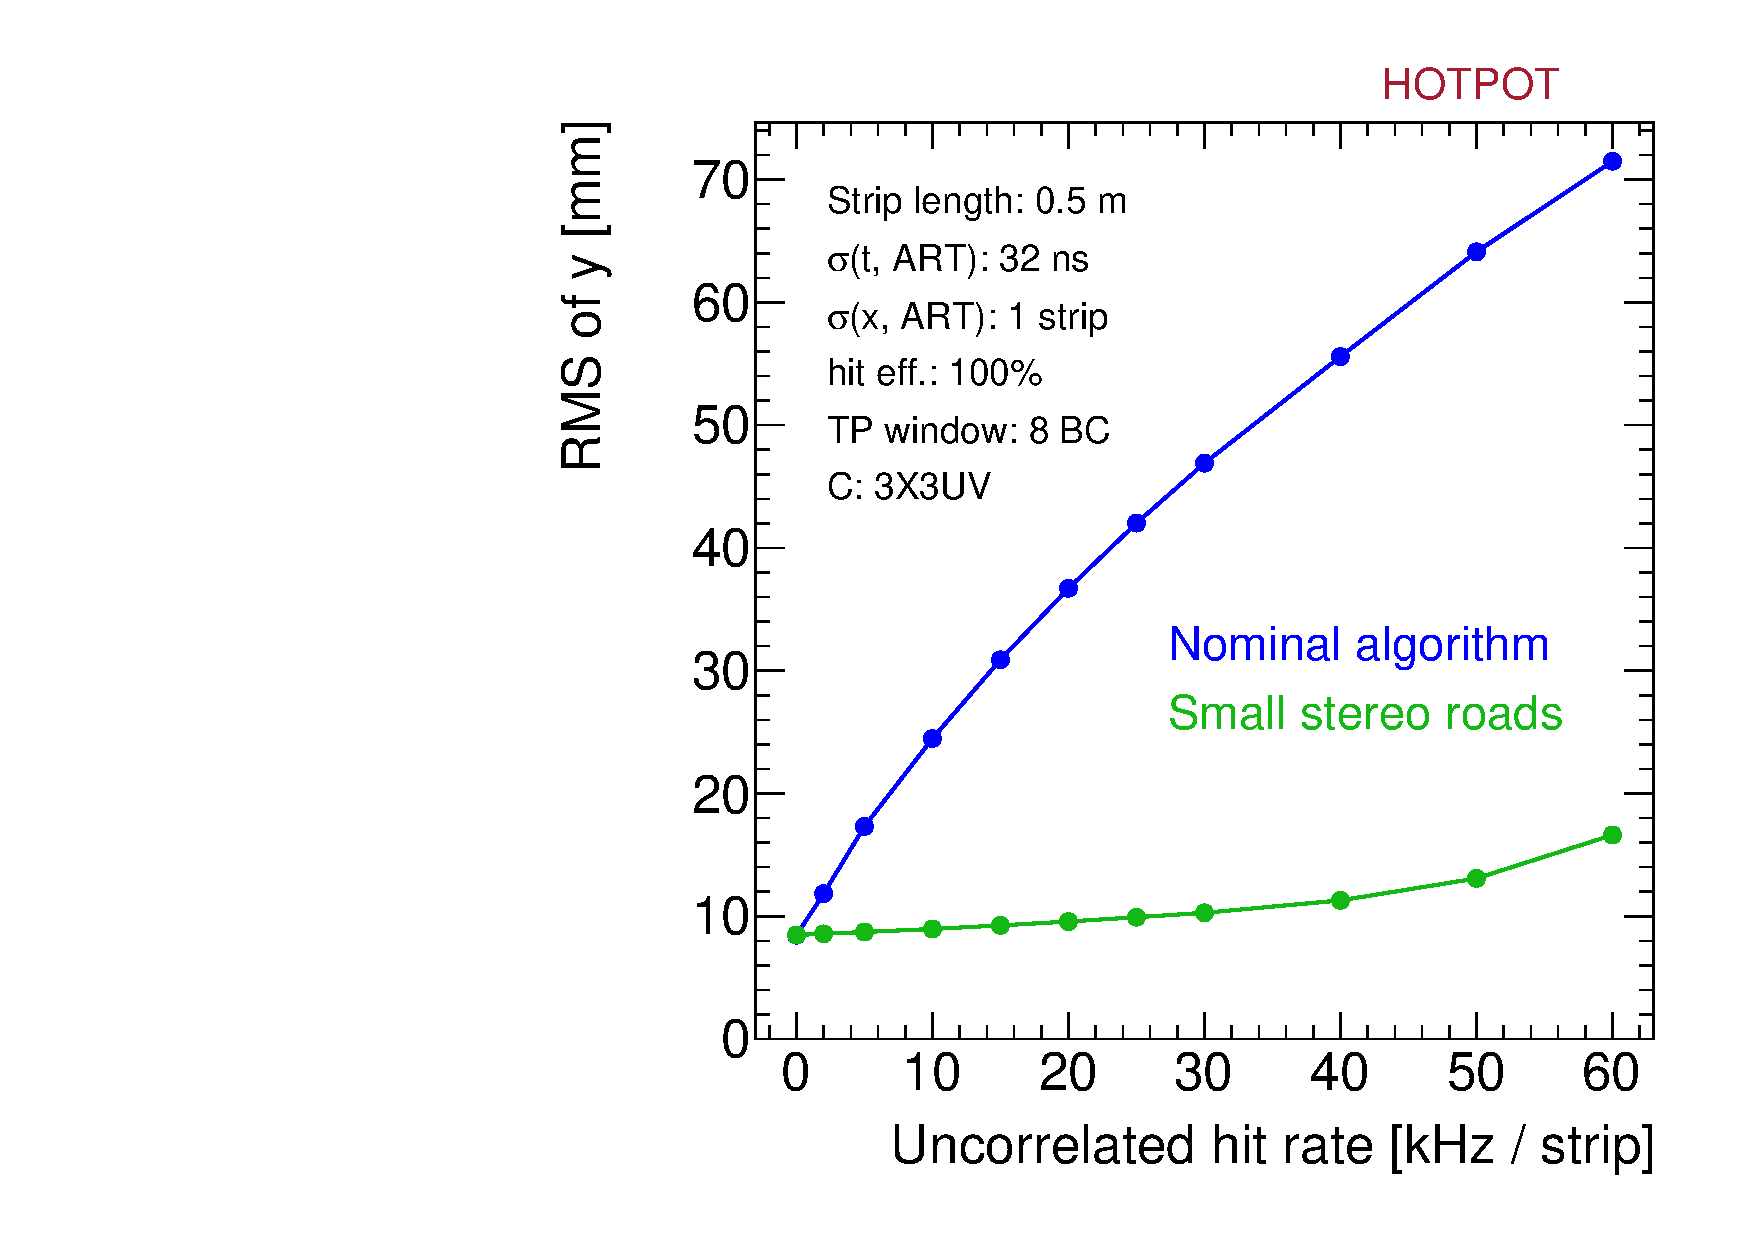
\includegraphics[width=0.48\textwidth]{figures/rms_y_small_vs_rate.pdf}
    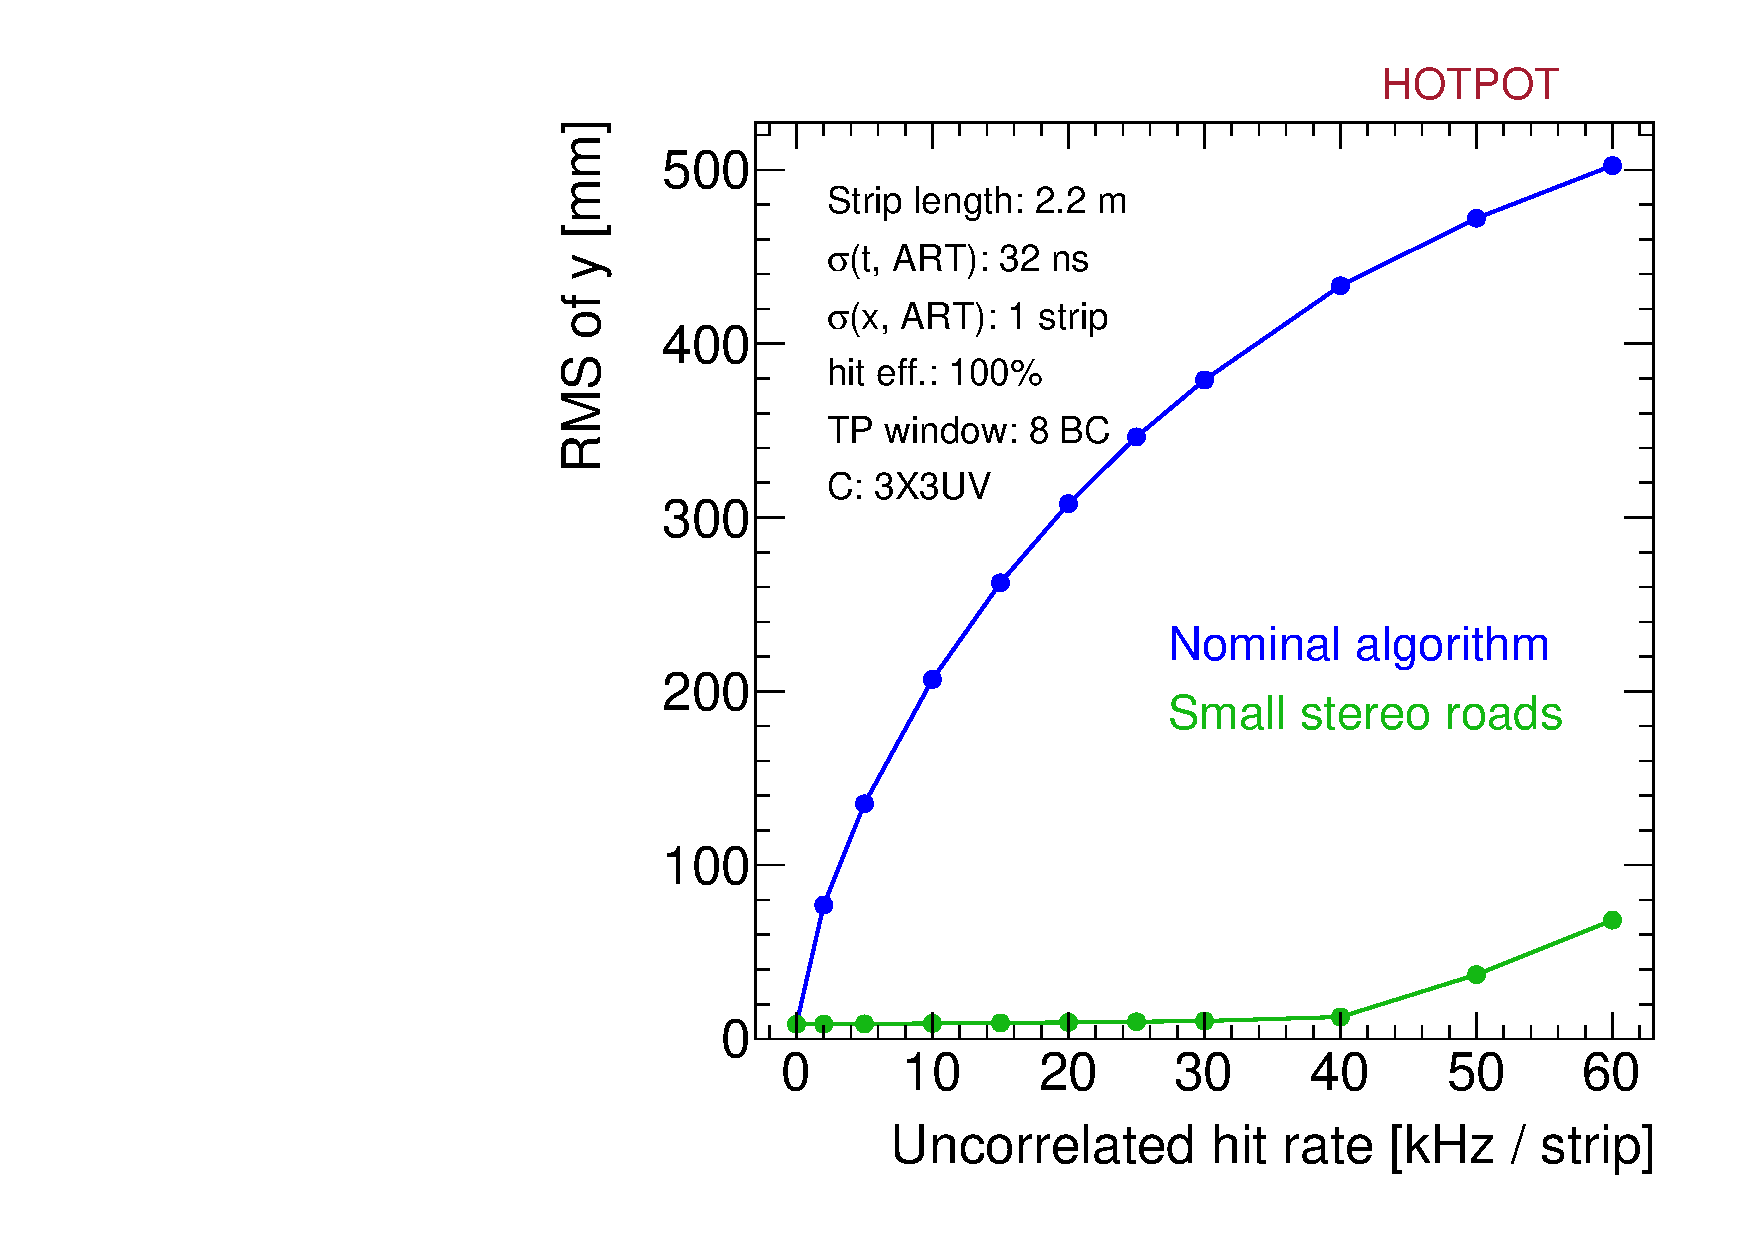
\includegraphics[width=0.48\textwidth]{figures/rms_y_large_vs_rate.pdf}
  \end{center}
  \vspace{-10pt}
  \caption{RMS of $y_\text{reco.} - y_\text{truth}$ for a strip size of 0.5m (left) and 2.2m (right) as a function of uncorrelated background rate. The RMS is calculated in the $3\sigma$ (99.7\%) range of the distribution.}
  \label{fig:rms_vs_rate}
\end{figure}

\begin{figure}[!htpb]
  \begin{center}
    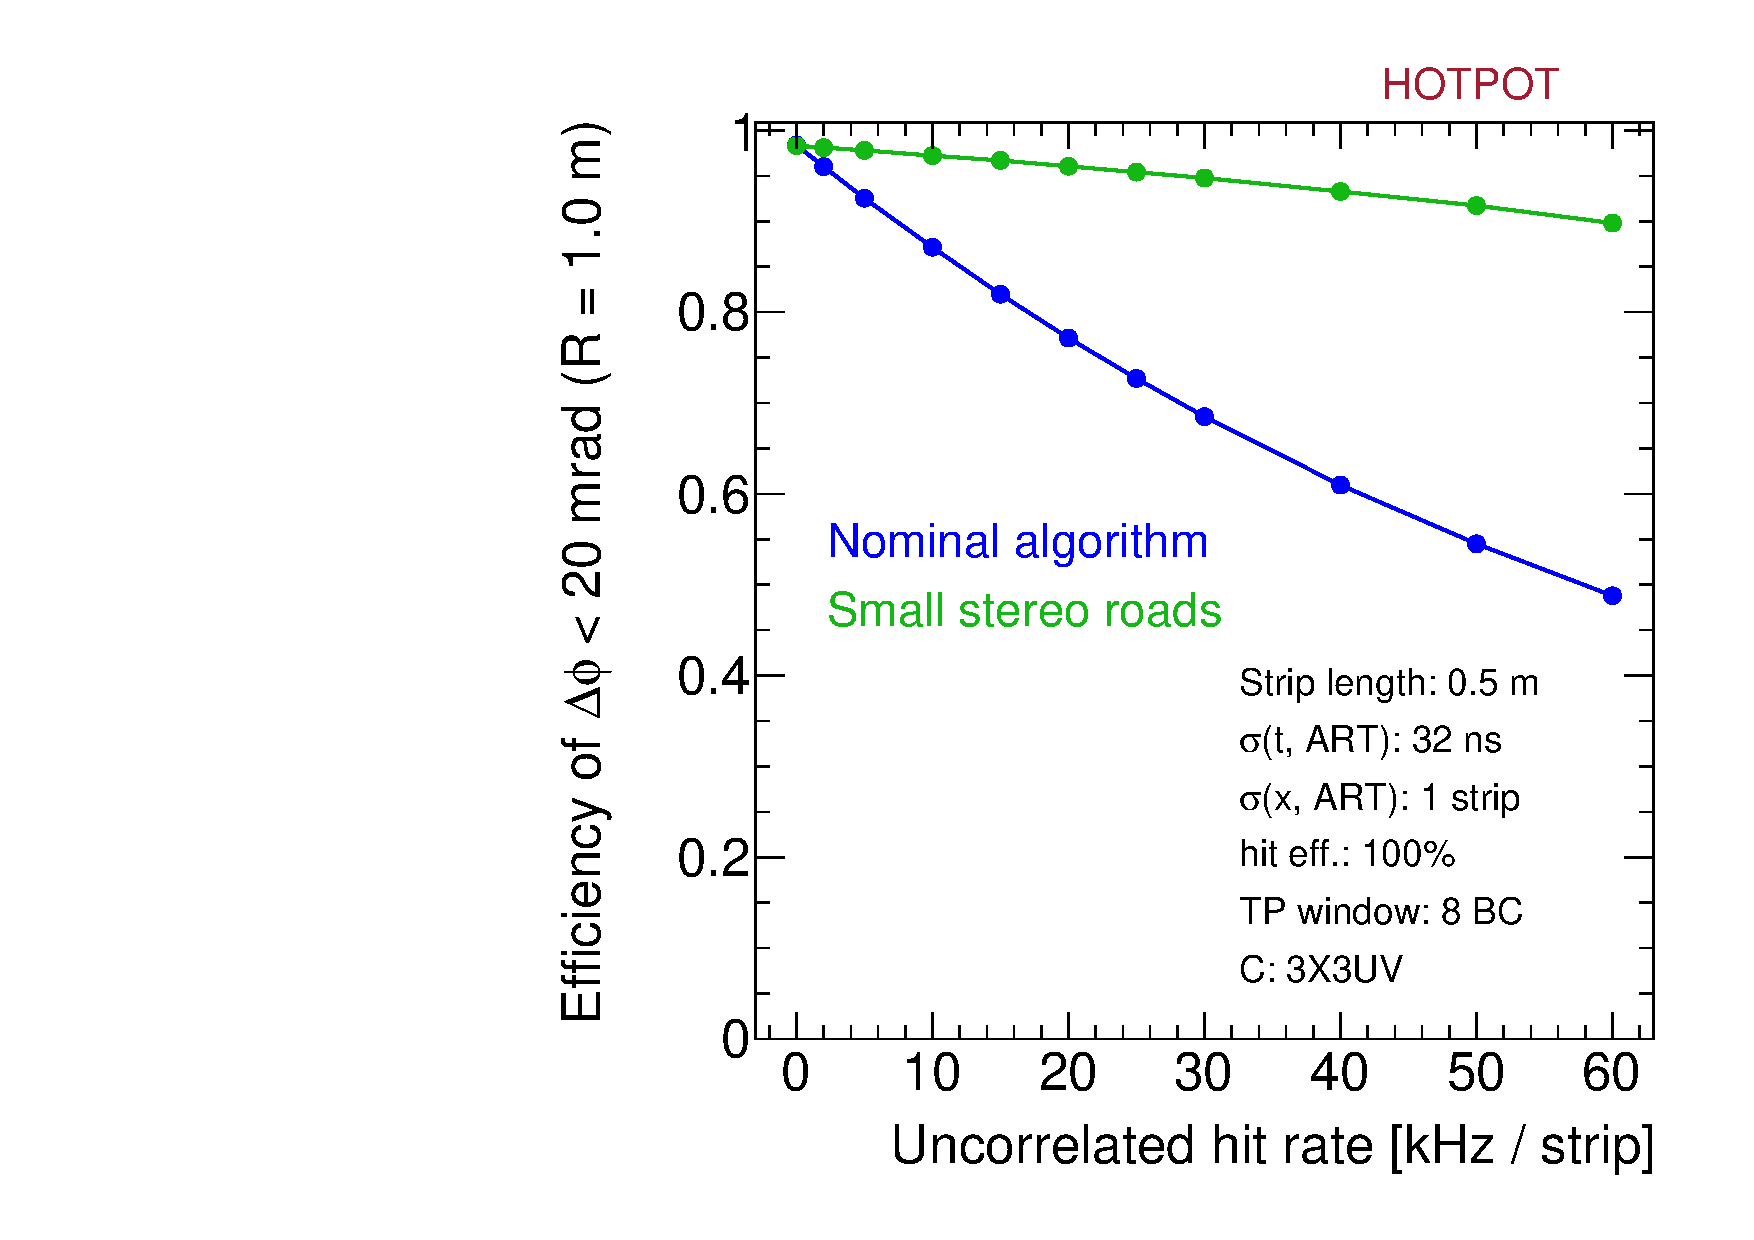
\includegraphics[width=0.48\textwidth]{figures/eff_phi_small_vs_rate.pdf}
    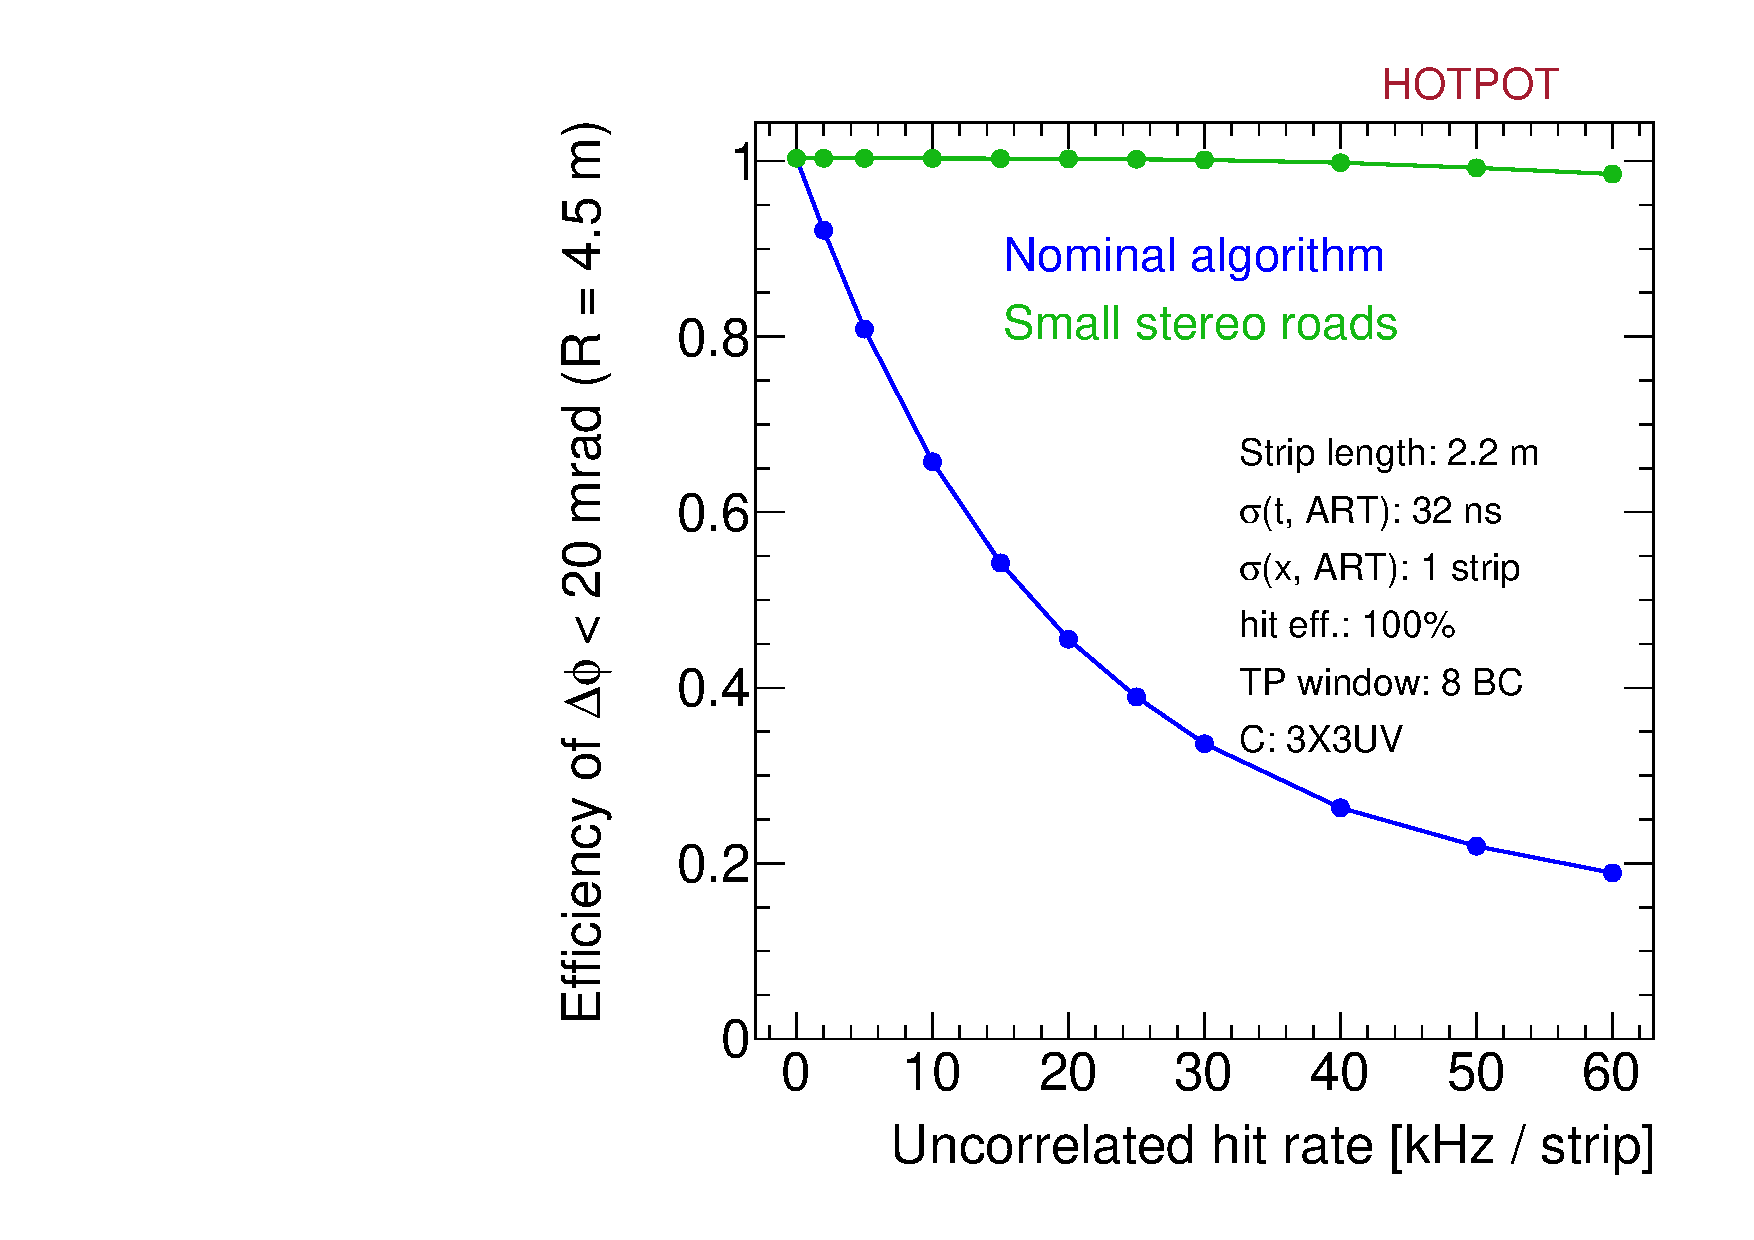
\includegraphics[width=0.48\textwidth]{figures/eff_phi_large_vs_rate.pdf}
  \end{center}
  \vspace{-10pt}
  \caption{Efficiency of $\phi_\text{reco.} - \phi_\text{truth} < 20$ mrad for a strip size of 0.5m (left) and 2.2m (right). $\phi_\text{reco.}-\phi_\text{truth}$ is calculated as $\frac{y_\text{reco.} - y_\text{truth}}{R}$, where $R$ is the distance from the beamline. $R$ is taken to be 1m for the small chamber and 4.5m for the large chamber.}
  \label{fig:eff_vs_rate}
\end{figure}

